\section{UV HWP Problems}
	
Throughout our calibration, we noticed that the angle $\theta$ for the UV-HWP that balances $\HH$ and $\VV$ production (which we might care about if we want to create say a Bell state like $\ket{\Phi^+}$) changes over time. To eliminate motion of the UV-HWP itself as a potential cause of the difference, we setup a series of ``drift experiments" to study how the proportion of $\HH$ to $\HH$ and $\VV$ drifted over time.

In these experiments, we essentially just configured the $\ket{\Phi^+}$ state to the best of our ability, and then began measuring $\HH$ and $\VV$ coincidence counts over extended periods of time. The results of the first experiment are shown in \cref{fig:DE0} and the second experiment's results can be found in \cref{fig:DE1}.

The UV-HWP is the only component in the setup that changes the proportion of $\HH$ and $\VV$ being produced, and so we strongly suspect that it is undergoing some change throughout our test. Personally, I believe this to be a temperature change. The 

\begin{figure}
	\centering
	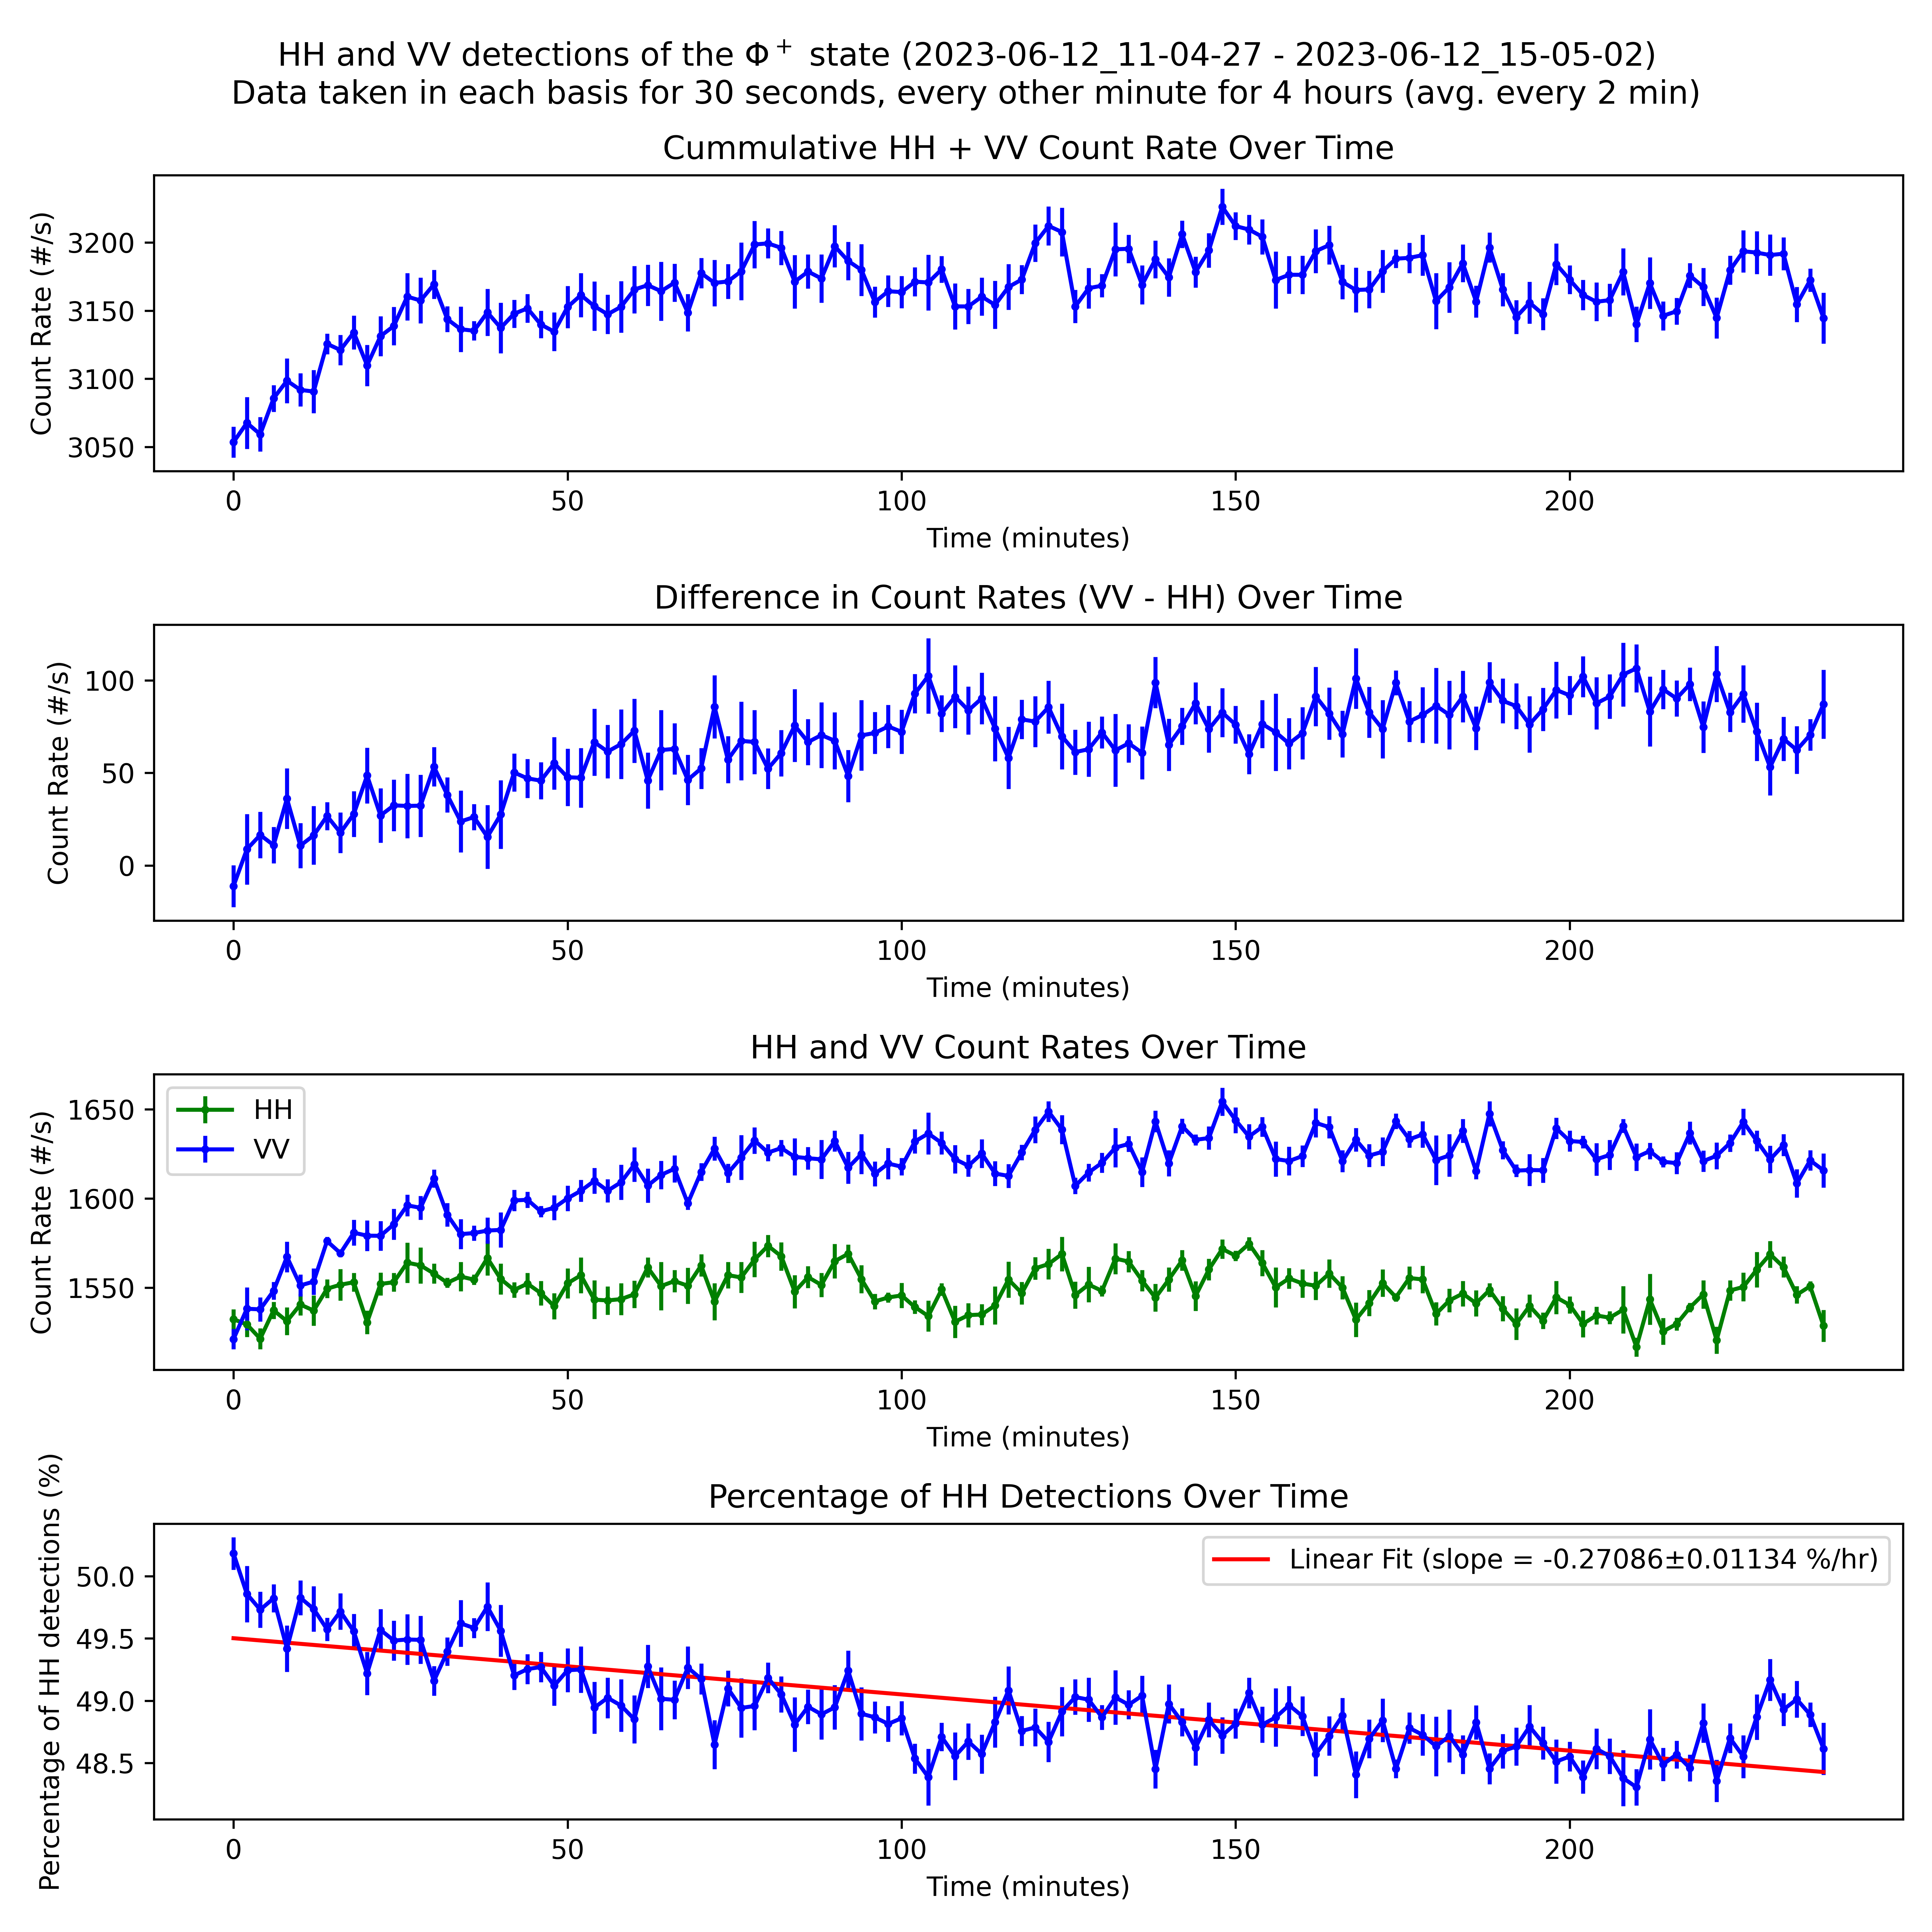
\includegraphics[width=\textwidth]{DE0_plot.png}	
	\caption{Results from the first drift experiment. Note the significant increase in overall production rates over the first 90 minutes. It Seems though that this figure could be explained by some overall preference for the $\VV$ state over time, since the middle plot shows $\HH$ counts effectively flatline throughout the experiment. To get a better grasp on this this data, we ran another experiment shortly after this one with the exact same setup, but for 5 hours.}
	\label{fig:DE0}
\end{figure}

\begin{figure}
	\centering
	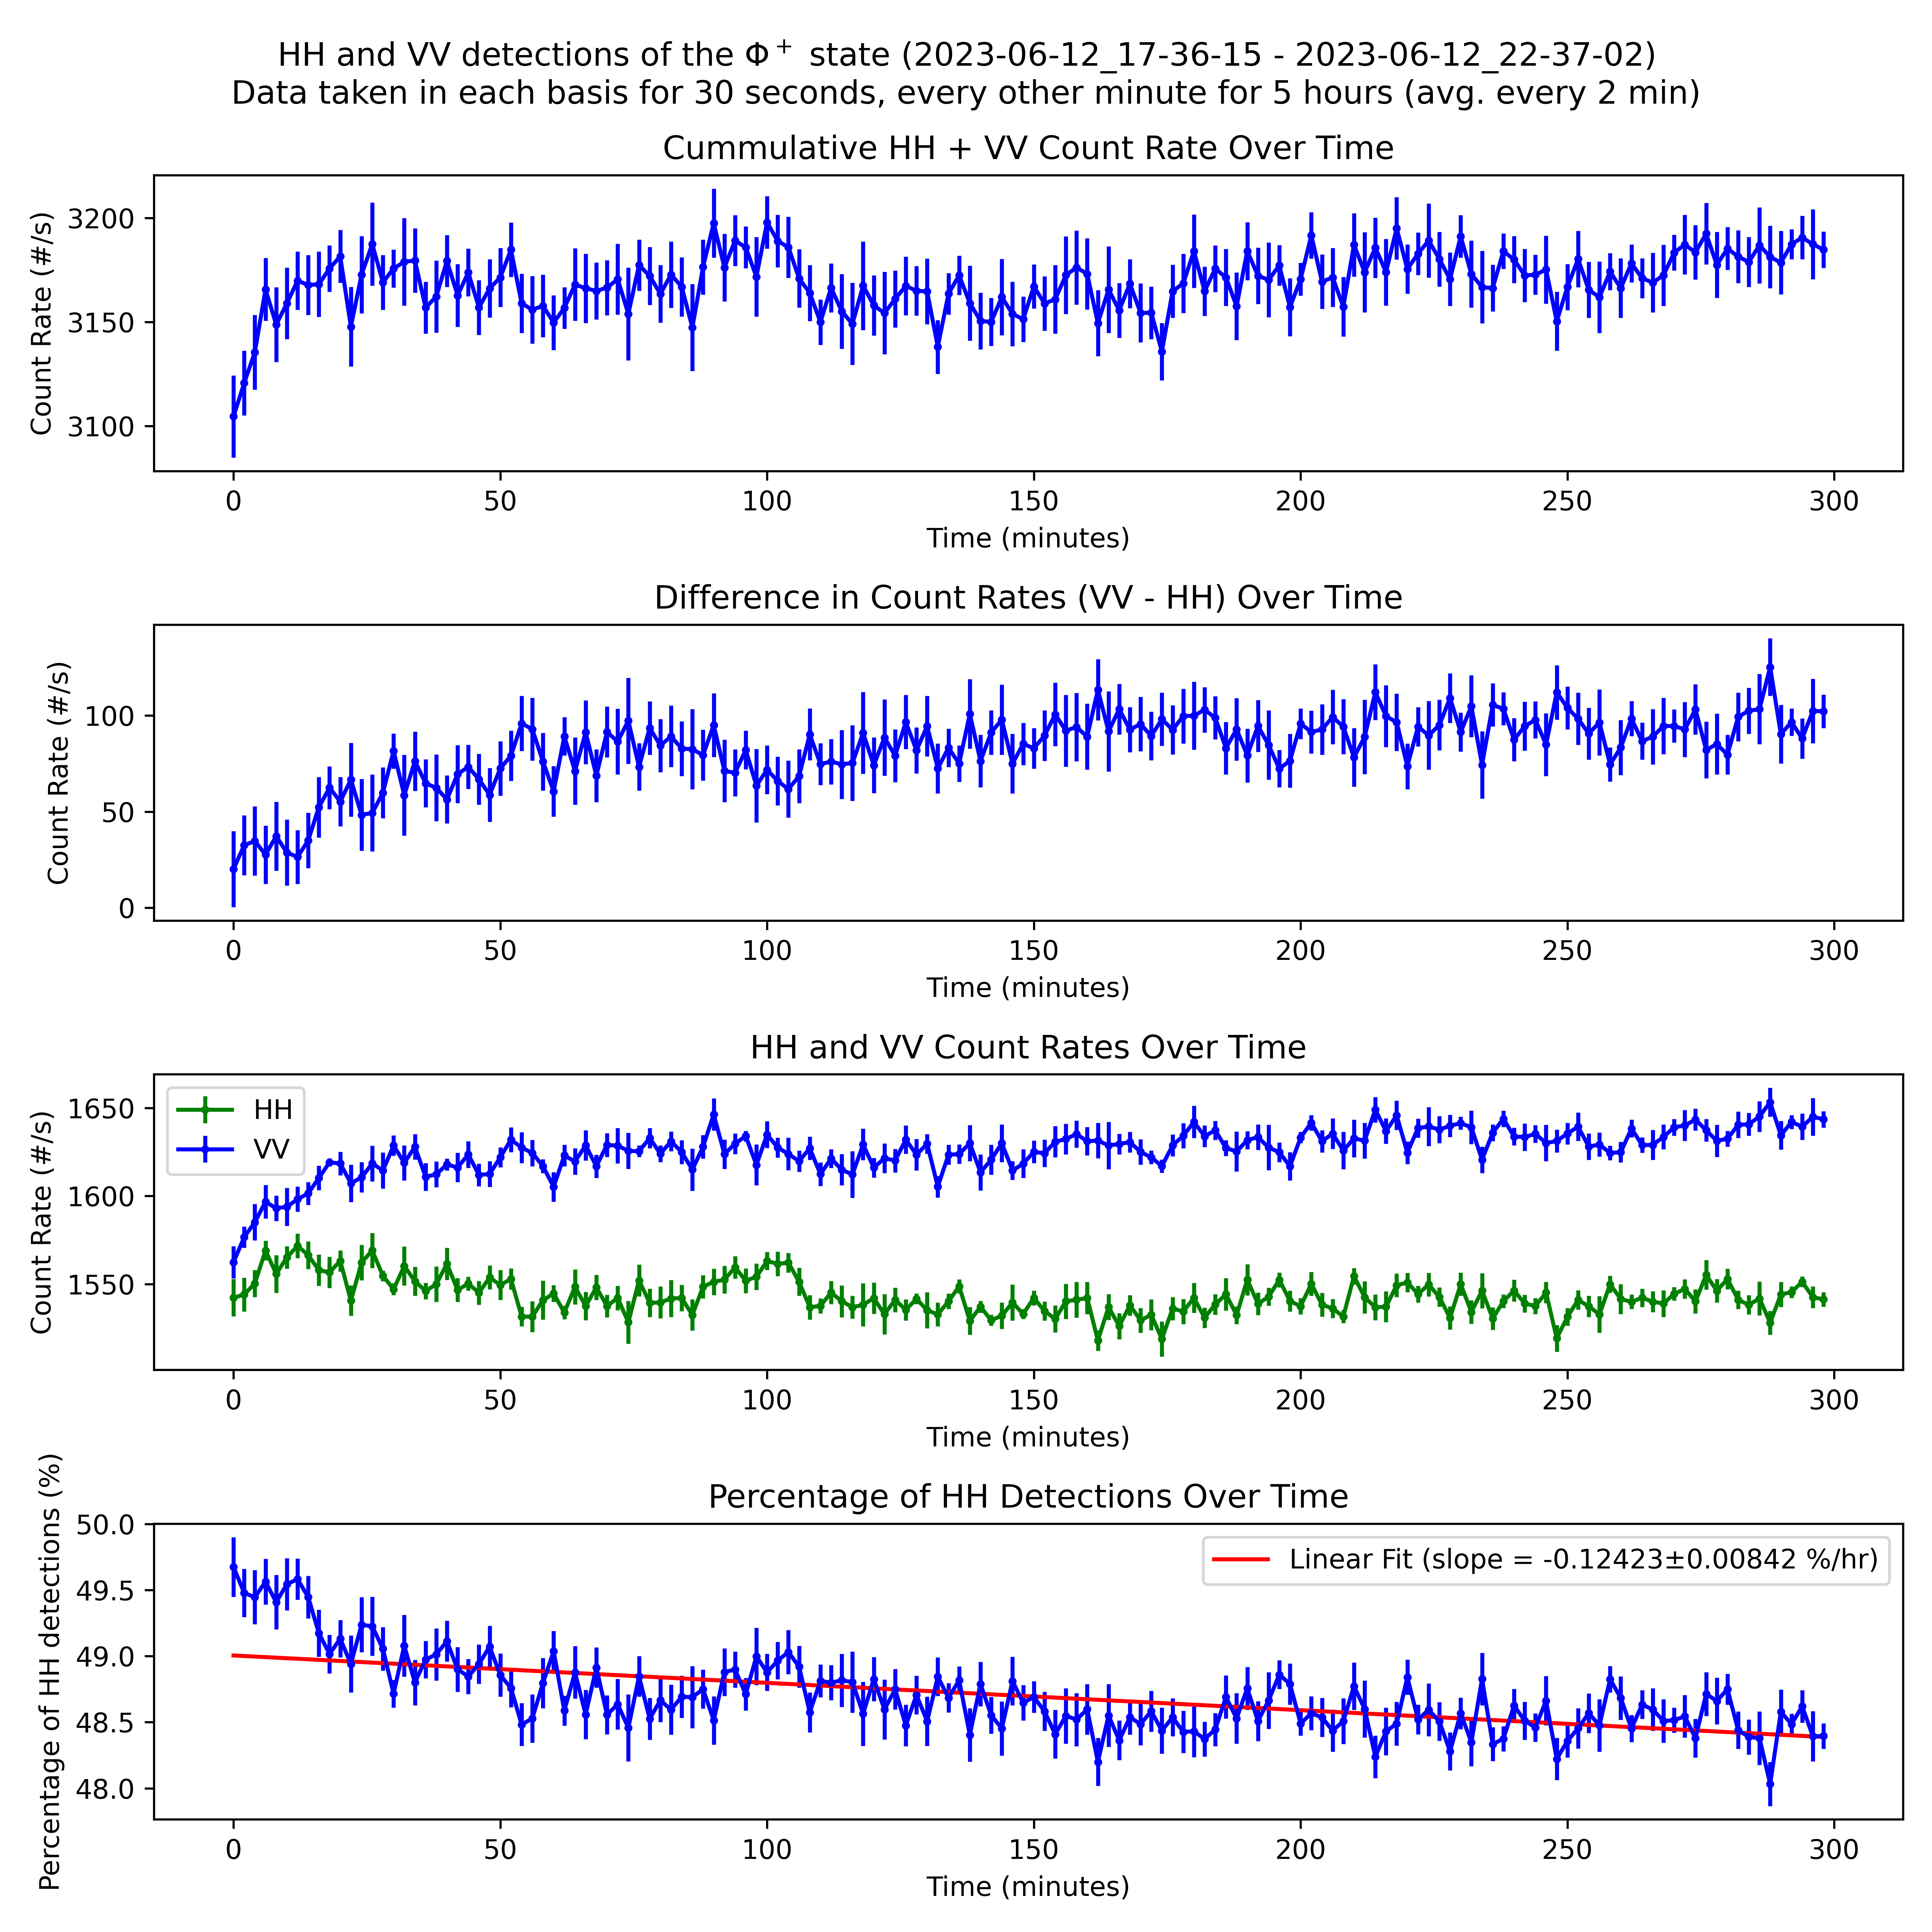
\includegraphics[width=\textwidth]{DE1_plot.png}
	\caption{The results of the second drift experiment we ran. Note that this was shortly after the first, and so if we believe temperature to be a factor, these plots should indicate that the components were already warm. Indeed, we see most of the values in these plots reaching equilibrium much faster than in \cref{fig:DE0}. The most provocative feature of this plot is that we see the relative ratio of $\HH$ to $\VV$ production changing \textit{after} the overall production rate has stabilized. This indicates that it likely is some (perhaps temperature-related) change in the UV-HWP causing the bias towards $\VV$ production, rather than just some kind of overall preference for excess $\VV$ production over time.}
	\label{fig:DE1}
\end{figure}


\subsection{Modeling the Issue}

If we believe that temperature affects the path length of the light in the crystal, then we can model the extra retardance applied to the vertical component with a \textit{small} phase error term $\gamma > 0$, so that the UV HWP will have a jones matrix
\begin{equation}
	\UVHWP = \begin{pmatrix}
		1 & 0 \\ 0 & -e^{-i\gamma}
	\end{pmatrix}
\end{equation}
Then the expanded expression when this plate is rotated to an angle $\theta$ from the horizontal becomes
\begin{align}
	\UVHWP(\theta) &= R\;\UVHWP\; R^\dagger \\
	&= \begin{pmatrix}
		\cos^2\theta - e^{-i\gamma}\sin^2\theta & (1+e^{-i\gamma})\cos\theta\sin\theta \\
		(1+e^{-i\gamma})\cos\theta\sin\theta & \sin^2\theta - e^{-i\gamma}\cos^2\theta
	\end{pmatrix}
\end{align}
And so the light from our laser becomes the state
\begin{equation}
	\UVHWP\H = \begin{pmatrix}
		\cos^2\theta - e^{-i\gamma}\sin^2\theta \\ (1+e^{-i\gamma})\cos\theta\sin\theta
	\end{pmatrix}
\end{equation}
And the probability of measuring this state to be in the state $\H$ or $\V$ (equal to the probability of measuring $\VV$ or $\HH$, respectively) is
\begin{align}
	P(\H) = P(\VV) &=1-\frac{1}{2}\sin^2(2\theta)(1+\cos\gamma)\\
	P(\V) = P(\HH) &=\frac{1}{2}\sin^2(2\theta)(1+\cos\gamma)
\end{align}
You'll notice that both these probabilities will have extrema at $\theta = n\cdot 45^\circ$ for $n\in\mathbb{Z}$ no matter what the value of $\gamma$ is. However, if we are doing something a bit more complex like say fine-tuning the balance of $\H$ and $\V$ states, we end up caring much more about $\gamma$.

Ignoring the fact that the quartz plate will reflect vertically and horizontally polarized light at different rates, we can pretend that the ratio of $\H$ to $\V$ will be perfectly balanced at the angle $\theta=\pi/8$ and $\sin^2(2\theta) = \frac{1}{2}$. One interesting prediction from the above equations is that as $\gamma\neq 0$, since $\cos$ is even and decreasing around the origin, we will see $P(\V)=P(\HH)$ decrease, and $P(\H)=P(\VV)$ increase, which is exactly what \cref{fig:DE0} and \cref{fig:DE1} show us experimentally.

In fact, using our experimental data we can even make a back-of-the envelope calculation for what $\gamma$ in our setup must be. Making the same assumption as above, that $\theta=\pi/8$ balances $\H$ and $\V$, then we can set $P(\V)=\frac{1}{2}-\delta$ for some real percentage error $\delta > 0$ and solve for the phase error $\gamma$. This leaves us with
\begin{align}
	P(\V)=\frac{1}{4}(1+\cos\gamma) &= \frac{1}{2} - \delta \\
	\gamma &= \arccos(1 - 4\delta)
\end{align}
In our experiment, we saw the $\HH$ counts drop by about $\delta \approx 1.5\%$ throughout the test, indicating a phase error of $\gamma\approx 0.348\approx 20^\circ$ which can also be expressed as $\frac{\gamma}{2\pi} = 0.055\lambda$ which is really quite a significant difference!

\subsection{Temperature Changes}

One hypothesis we explored was that possibility that the heating of the quartz plate by our laser was causing the plate to expand, changing the path length of light through the plate and thus the retardance. However, since the phase shift is linear with the path length and the thermal expansion coefficient of quartz is like\footnote{https://www.heliosquartz.com/prodotti/proprieta-del-quarzo/?lang=en}\textsuperscript{,}\footnote{http://www.mt-berlin.com/frames\_cryst/descriptions/quartz\%20.htm} $\epsilon \approx 5.5\times 10^{-7} \;\ut{K}^{-1}$ then the phase shift with respect to a change in temperature will look like $\phi = \phi_0(1+\epsilon\Delta T)$ or $\gamma = \Delta \phi = \phi_0\epsilon\Delta T$. For our HWP where $\phi_0=\pi$ this means that to achieve a phase difference $\gamma$ we require a temperature change $\Delta T= \gamma/\pi\epsilon$ and perhaps you can see the problem when noting the order of magnitude of $\epsilon$. To achieve $\gamma=0.348\;\ut{rad}$ we would require a temperature change of $\Delta T \approx 200,000 \;\ut{K}$.

But that's a bit of a silly approximation, since wave plates employ all kinds of tricks and gimmicks and so it's a bit disingenuous to model them as slabs of quartz. The other (probably better) way to go about this approximation is by noting a typical thermal dependence for zero order wave plates\footnote{https://www.newport.com/n/introduction-to-waveplates} being something like $\epsilon=0.0001\;\lambda\;\utx{C}{-1}$ and then we can directly compare with the observed retardance error of $0.055\;\lambda$ to get a required temperature change of about $550\;\ut{K}$, which is still not very realistic for our circumstances.

These calculations suggest that temperature changes in the quartz will not be enough to appreciably affect the drift of the $\H$ : $\V$ balance that we are measuring.

\subsection{Laser Drift}

Another factor that affects the retardance of a wave plate is the wave length of light passing through it. The wave length of our laser should be centered around $405\;\ut{nm}$, but nothing is ever perfect. Luckily, ThorLabs provides great data sheets on their HWPs\footnote{https://www.thorlabs.com/newgrouppage9.cfm?objectgroup\_id=711}, a plot of which is shown in \cref{fig:405nm wp wavelen vs retardance}.
\begin{figure}[ht]
	\centering
	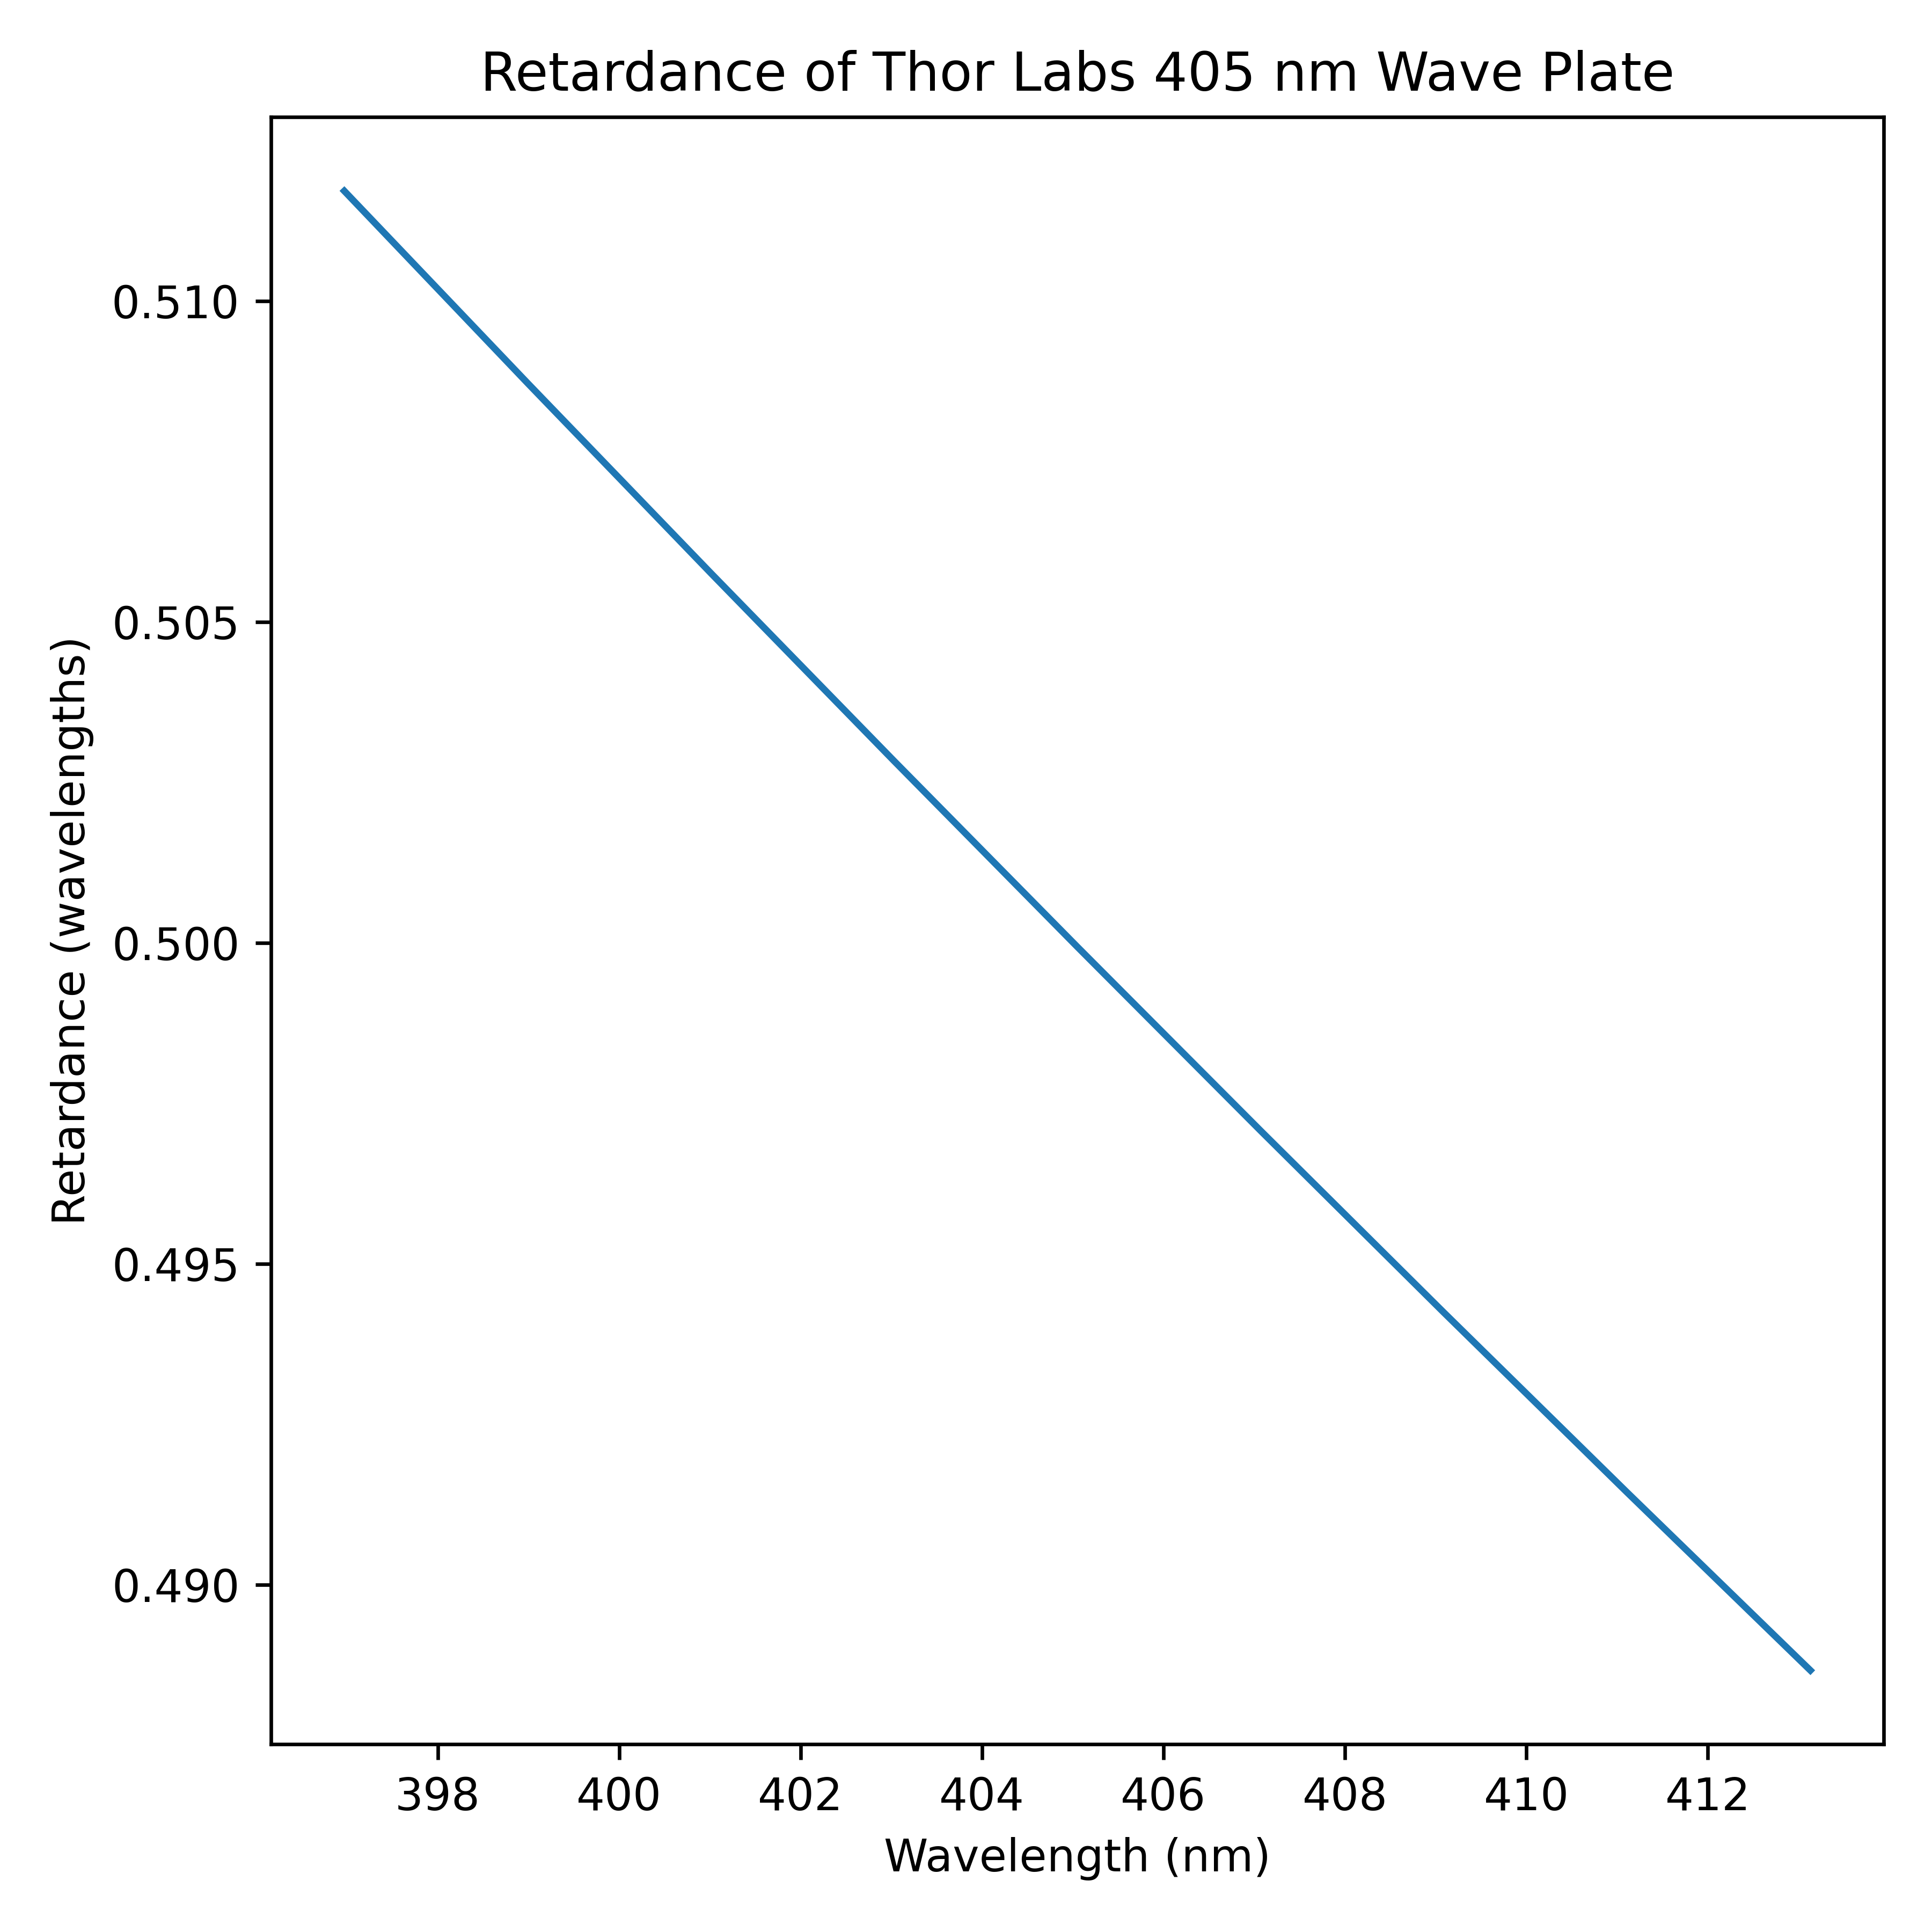
\includegraphics[width=\textwidth]{405_WP_retardance.png}
	\caption{Plotted data from ThorLabs showing the retardance in of the ThorLabs zero-order quartz crystal 405 nm wave plate (measured in wavelengths) versus the wavelength of light.}
	\label{fig:405nm wp wavelen vs retardance}
\end{figure}
I've zoomed in on the most relevant part of the plot here, where it is clear a deviation of $\pm5\;\ut{nm}$ from the central wavelength of $405\;\ut{nm}$ could easily cause a retardance difference of $0.055\;\lambda$, explaining the percentage difference that we see. However, after discussing these ideas with Prof. Lynn, she believes this would be well outside of the drift of a laser with these specifications. Measurements on the grating spectrometer from fifteen years ago suggest temperature related drift was $<0.1{}^\circ\ut{A}$, however their relevance is of suspicion as the measurements are fifteen years old.








	